\subsection{Reinitializing the Level Set}

The goal of the reinitializing step is to make sure that the gradient of the level set is always a unit vector, i.e the length is 1. To do this we will use a method called fast sweeping, which sweeps and propagates the solution of an iterative approach in different directions. Before we go into detail about the fast sweeping algorithm itself, let us write down and evaluate tha gradient of $\phi$ and the Eikonal equation in two dimensions

\begin{equation}
\nabla \phi = (\frac{\partial \phi}{\partial x}, \frac{\partial \phi}{\partial y})
\end{equation}

\begin{equation}
\begin{split}
|\nabla \phi| &= \sqrt{{(\frac{\partial \phi}{\partial x})}^2 + {(\frac{\partial \phi}{\partial y})}^2}  = 1
\end{split}
\label{evaleiokanl}
\end{equation}
\noindent
We can now turn Equation \ref{evaleiokanl} into an discrete version and therefore making it possible to solve it iteratively. Let us approximate the partial derivatives with backward differences

\begin{equation}
\begin{split}
\frac{\partial \phi}{\partial x} &\approx \frac{\phi_{i,j} - \phi_{i-1,j}}{\Delta x} \\
\frac{\partial \phi}{\partial y} &\approx \frac{\phi_{i,j} - \phi_{i,j-1}}{\Delta x}
\end{split}
\label{phiapproxeq}
\end{equation}
\noindent
If we square both the left and right hand side of Equation \ref{evaleiokanl} and use the approximations of the partial derivatives, we get

\begin{equation}
\begin{split}
{(\frac{\phi_{i,j} - \phi_{i-1,j}}{\Delta x})}^2 + {(\frac{\phi_{i,j} - \phi_{i,j-1}}{\Delta x})}^2 &= 1 \\ 
({\phi_{i,j}}^2 - 2\phi_{i,j}\phi_{i-1,j} + {\phi_{i-1,j}}^2) + 
({\phi_{i,j}}^2 - 2\phi_{i,j}\phi_{i,j-1} + {\phi_{i,j-1}}^2)
&= {\Delta x}^2 \\
2{\phi_{i,j}}^2 - 2\phi_{i,j}(\phi_{i-1,j} + \phi_{i,j-1}) + {\phi_{i-1,j}}^2 + {\phi_{i,j-1}}^2 - {\Delta x}^2 &= 0 \\
{\phi_{i,j}}^2 - \phi_{i,j}(\phi_{i-1,j} + \phi_{i,j-1}) + \frac{{\phi_{i-1,j}}^2 + {\phi_{i,j-1}}^2 - {\Delta x}^2}{2} &= 0
\end{split}
\label{phisimplified}
\end{equation}
\noindent
To simplify things, let us store the non $\phi_{i,j}$ parts in temporary variables
\begin{equation}
\begin{split}
b &= \phi_{i-1,j} + \phi_{i,j-1} \\
c &= \frac{{\phi_{i-1,j}}^2 + {\phi_{i,j-1}}^2 - {\Delta x}^2}{2}
\end{split}
\label{variablesreinit}
\end{equation}
\noindent
Equation \ref{phisimplified} can then be put on the form

\begin{equation} 
{\phi_{i,j}}^2 - \phi_{i,j} b + c = 0
\end{equation}

which is a standard quadratic equation. Rearranging the terms we get

\begin{equation} 
\begin{split}
{\phi_{i,j}}^2 - \phi_{i,j} b + c &= 0 \\
{(\phi_{i,j} - \frac{b}{2})}^2  = b^2 - c \\
\phi_{i,j} =  \frac{b}{2} \pm \sqrt{b^2 - c}
\end{split}
\label{solvephi}
\end{equation}
\noindent
If $b^2 - c < 0$, we do not update $\phi_{i,j}^{n+1}$. If $b^2 - c > 0$, Equation \ref{solvephi} has two real solutions ${\phi_{i,j}}^a$ and ${\phi_{i,j}}^b$. We pick the smaller value of the two as our solution. 

\begin{equation}
{\phi_{i,j}}^{new} = min({\phi_{i,j}}^a, {\phi_{i,j}}^b)
\end{equation}
\noindent
Another condition we use is that new solution to ${\phi_{i,j}}^{new}$ has to be smaller than the previous value ${\phi_{i,j}}^{n}$. This is why it was important to pick $D >> \Delta x$. It means that we are only propagating the level set from the surface and inwards/outwards and not from the center of the fluid towards the surface.

\begin{equation}
{\phi_{i,j}}^{n+1} = 
\left\{
\begin{array}{ll}
{\phi_{i,j}}^{new} & \mbox{if ${\phi_{i,j}}^{new} < {\phi_{i,j}}^{n}$} \\
{\phi_{i,j}}^{n} & \mbox{if ${\phi_{i,j}}^{new} > {\phi_{i,j}}^{n}$}
\end{array}
\right.
\end{equation}
\noindent
Now that we have an iterative way of solving the Eikonal equation, let us talk more about the fast sweeping method. Fast sweeping for solving the Eikonal equation was introduced by Zhao\cite{zhao}. The fundamentals of the method are that you sweep your domain in every possible direction which tells you in which order to update the cells. In a two dimensional case, there are only four different directions:

\begin{itemize}
\item left to right, bottom to top
\item left to right, top to bottom
\item right to left, bottom to top
\item right to left, top to bottom
\end{itemize}
\noindent
Depending on the sweeping order, the approximation of the partial derivatives in Equation \ref{phiapproxeq} is different. The goal with fast sweeping is to use updated data from the same sweep and therefore have faster convergence. For example, if we are sweeping from left to right, it makes sense to approximate the horizontal partial derivative with $\phi_{i,j} - \phi_{i-1,j}$ since $\phi_{i-1,j}$ was just updated. However, if we are sweeping from right to left, then it is better to approximate the horizontal partial derivative with $\phi_{i,j} - \phi_{i+1,j}$. We need to take this into account when we are solving Equation \ref{solvephi}.

\begin{equation}
\frac{\partial \phi}{\partial x} \approx
\left\{
\begin{array}{ll}
\frac{\phi_{i,j} - \phi_{i-1,j}}{\Delta x} & \mbox{if horizontal sweeping is left to right} \\
\frac{\phi_{i,j} - \phi_{i+1,j}}{\Delta x} & \mbox{if horizontal sweeping is right to left} \\
\end{array}
\right.
\end{equation}

\begin{equation}
\frac{\partial \phi}{\partial y} \approx
\left\{
\begin{array}{ll}
\frac{\phi_{i,j} - \phi_{i,j-1}}{\Delta x} & \mbox{if vertical sweeping is bottom to top} \\
\frac{\phi_{i,j} - \phi_{i,j+1}}{\Delta x} & \mbox{if vertical sweeping is top to bottom} \\
\end{array}
\right.
\end{equation}

Figure \ref{sweeppic} shows an example of the update order when sweeping from left to right and bottom to right.

\begin{figure}[ht!]
\centering
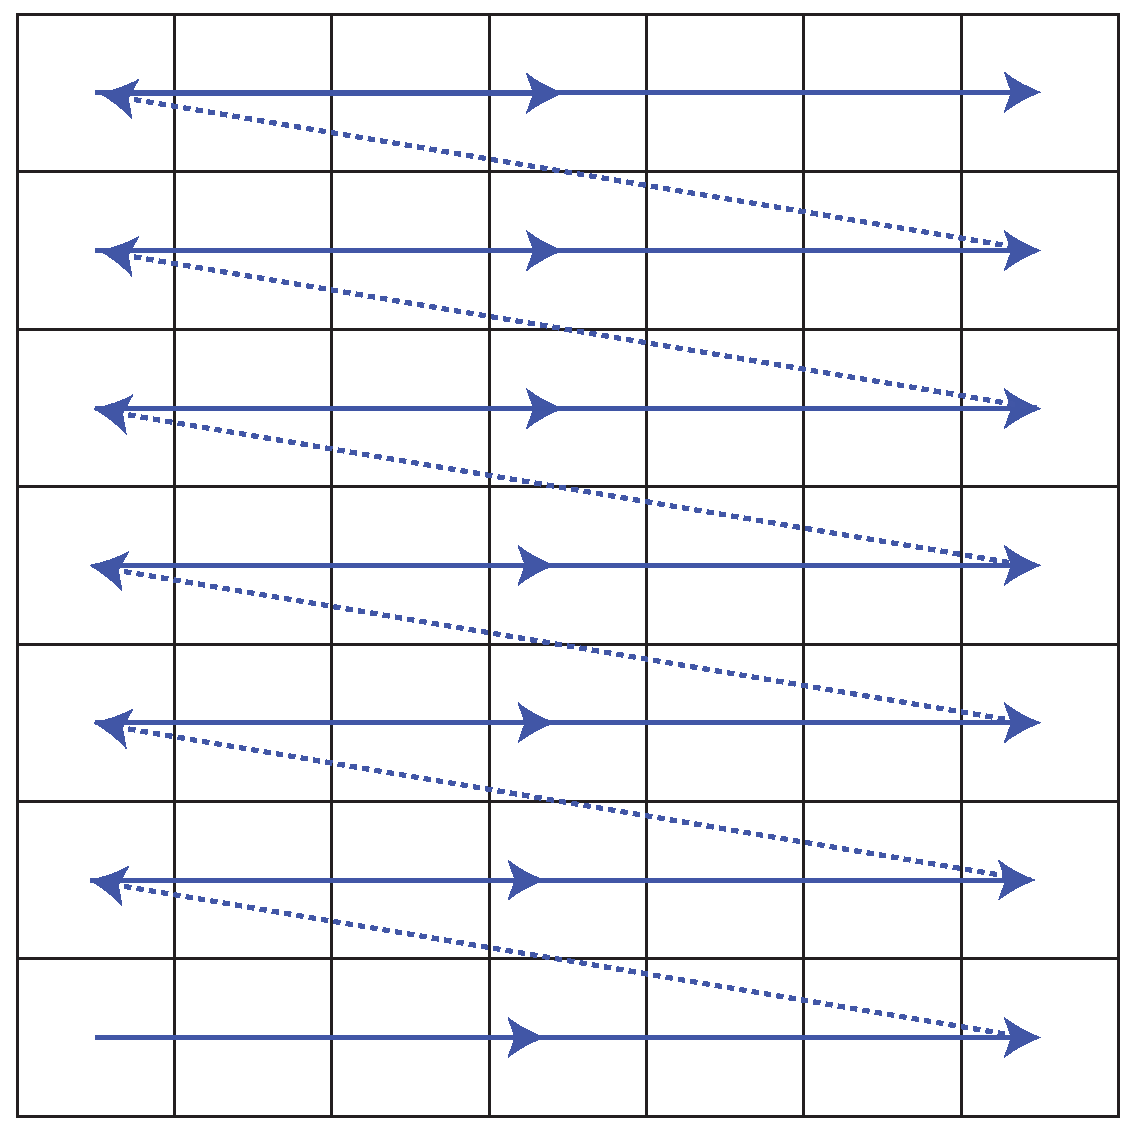
\includegraphics[width=80mm]{img/sweep.pdf}
\caption{Left to right, bottom to top sweeping order. In an iterative solver, the cells are updated in the order of the blue arrows.}
\label{sweeppic}
\end{figure}
